% answers.tex —— 2003 年·河南卷 · 参考答案与详细解析片段
% 由 tools/generate_projects.py 依来源总账自 2003/2003_数学真题_河南_试题.md + 2003/2003_数学真题_河南_解析正文.md + 2003/2003_数学真题_河南_答案要点.md 生成，勿手改（改源 MD 后重跑）


\begin{gktip}
固定源 PDF 仅含 4 页题面，无官方答案与解析页。以下各题均依据题面独立复算并经双角色交叉核验；第 16、17、19 题的图形在 LaTeX 工程中统一采用 TikZ 矢量重绘。
\end{gktip}

\begin{answer}
\gksolhead{1}{}

\textbf{题目}：

若圆 $C$ 与圆 $(x+2)^2 + (y-1)^2 = 1$ 关于原点对称，则圆 $C$ 的方程为\mbox{（　　）}

（A）$(x-2)^2 + (y+1)^2 = 1$　　（B）$(x-2)^2 + (y-1)^2 = 1$

（C）$(x-1)^2 + (y+2)^2 = 1$　　（D）$(x+1)^2 + (y-2)^2 = 1$

\Needspace{4\baselineskip}
\textbf{解析}

圆 $(x+2)^2 + (y-1)^2 = 1$ 的圆心坐标为 $(-2, 1)$，半径为 $r = 1$。
\Needspace{5\baselineskip}
设圆心 $(-2, 1)$ 关于原点 $(0, 0)$ 对称的点为 $(x_0, y_0)$，则：
\nopagebreak[4]
\[x_0 = -(-2) = 2, \quad y_0 = -(1) = -1.\]
所求圆 $C$ 的圆心为 $(2, -1)$，半径仍为 $r = 1$。
\Needspace{5\baselineskip}
因此，圆 $C$ 的方程为：
\nopagebreak[4]
\[(x - 2)^2 + (y + 1)^2 = 1.\]

故选 A。

\gkanswer{答案：A}

\end{answer}
\begin{answer}
\gksolhead{2}{}

\textbf{题目}：

抛物线 $y = ax^2$ 的准线方程是 $y = 2$，则 $a$ 的值为\mbox{（　　）}

（A）$\dfrac{1}{8}$　　（B）$-\dfrac{1}{8}$　　（C）8　　（D）$-8$

\Needspace{4\baselineskip}
\textbf{解析}

\Needspace{5\baselineskip}
抛物线方程 $y = ax^2$ 化为标准方程为：
\nopagebreak[4]
\[x^2 = \frac{1}{a} y.\]
其顶点在原点，对称轴为 $y$ 轴，焦点在 $y$ 轴上。
\Needspace{5\baselineskip}
由标准方程 $x^2 = 2py$ 的准线方程为 $y = -\dfrac{p}{2}$ 可知，抛物线 $x^2 = \dfrac{1}{a} y$ 的准线方程为：
\nopagebreak[4]
\[y = -\frac{1}{4a}.\]
\Needspace{5\baselineskip}
由题意，准线方程是 $y = 2$，故：
\nopagebreak[4]
\[-\frac{1}{4a} = 2 \implies 4a = -\frac{1}{2} \implies a = -\frac{1}{8}.\]

故选 B。

\gkanswer{答案：B}

\end{answer}
\begin{answer}
\gksolhead{3}{}

\textbf{题目}：

已知 $x \in \left(-\dfrac{\pi}{2}, 0\right)$，$\cos x = \dfrac{4}{5}$，则 $\tan 2x =$\mbox{（　　）}

（A）$\dfrac{7}{24}$　　（B）$-\dfrac{7}{24}$　　（C）$\dfrac{24}{7}$　　（D）$-\dfrac{24}{7}$

\Needspace{4\baselineskip}
\textbf{解析}

由 $x \in \left(-\dfrac{\pi}{2}, 0\right)$，可知 $x$ 为第四象限角，$\sin x < 0$。
\Needspace{5\baselineskip}
已知 $\cos x = \dfrac{4}{5}$，则：
\nopagebreak[4]
\[\sin x = -\sqrt{1 - \cos^2 x} = -\sqrt{1 - \left(\frac{4}{5}\right)^2} = -\frac{3}{5}.\]
\Needspace{5\baselineskip}
所以：
\nopagebreak[4]
\[\tan x = \frac{\sin x}{\cos x} = \frac{-3/5}{4/5} = -\frac{3}{4}.\]
\Needspace{5\baselineskip}
利用倍角公式：
\nopagebreak[4]
\[\tan 2x = \frac{2\tan x}{1 - \tan^2 x} = \frac{2 \times \left(-\dfrac{3}{4}\right)}{1 - \left(-\dfrac{3}{4}\right)^2} = \frac{-\dfrac{3}{2}}{1 - \dfrac{9}{16}} = \frac{-\dfrac{3}{2}}{\dfrac{7}{16}} = -\frac{24}{7}.\]

故选 D。

\gkanswer{答案：D}

\end{answer}
\begin{answer}
\gksolhead{4}{}

\textbf{题目}：

已知四边形 $ABCD$ 是菱形，点 $P$ 在对角线 $AC$ 上（不包括端点 $A, C$），则 $\vec{AP} =$\mbox{（　　）}

（A）$\lambda(\vec{AB} + \vec{AD})$，$\lambda \in (0, 1)$　　（B）$\lambda(\vec{AB} + \vec{BC})$，$\lambda \in \left(0, \dfrac{\sqrt{2}}{2}\right)$

（C）$\lambda(\vec{AB} - \vec{AD})$，$\lambda \in (0, 1)$　　（D）$\lambda(\vec{AB} - \vec{BC})$，$\lambda \in \left(0, \dfrac{\sqrt{2}}{2}\right)$

\Needspace{4\baselineskip}
\textbf{解析}

\Needspace{5\baselineskip}
在菱形 $ABCD$ 中，根据向量加法的平行四边形法则，对角线向量为：
\nopagebreak[4]
\[\vec{AC} = \vec{AB} + \vec{AD}.\]
因为点 $P$ 在对角线 $AC$ 上，且不包括端点 $A, C$，所以向量 $\vec{AP}$ 与 $\vec{AC}$ 同向共线，且模长满足 $0 < |\vec{AP}| < |\vec{AC}|$。
\Needspace{5\baselineskip}
因此存在唯一的实数 $\lambda \in (0, 1)$，使得：
\nopagebreak[4]
\[\vec{AP} = \lambda \vec{AC} = \lambda(\vec{AB} + \vec{AD}).\]

故选 A。

\gkanswer{答案：A}

\end{answer}
\begin{answer}
\gksolhead{5}{}

\textbf{题目}：

\Needspace{5\baselineskip}
设函数
\nopagebreak[4]
\[f(x) = \begin{cases} 2^{-x} - 1, & x \le 0, \\ x^{\frac{1}{2}}, & x > 0, \end{cases}\]
若 $f(x_0) > 1$，则 $x_0$ 的取值范围是\mbox{（　　）}

（A）$(-1, 1)$　　（B）$(-1, +\infty)$　　（C）$(-\infty, -2) \cup (0, +\infty)$　　（D）$(-\infty, -1) \cup (1, +\infty)$

\Needspace{4\baselineskip}
\textbf{解析}

分段函数 $f(x) = \begin{cases} 2^{-x} - 1, & x \le 0, \\ x^{\frac{1}{2}}, & x > 0. \end{cases}$
要求 $f(x_0) > 1$，分两种情况讨论：
\Needspace{5\baselineskip}
1. 当 $x_0 \le 0$ 时：
\nopagebreak[4]
\[2^{-x_0} - 1 > 1 \iff 2^{-x_0} > 2 \iff -x_0 > 1 \iff x_0 < -1.\]
   因为 $-1 \le 0$，所以此时解为 $x_0 \in (-\infty, -1)$。
\Needspace{5\baselineskip}
2. 当 $x_0 > 0$ 时：
\nopagebreak[4]
\[x_0^{\frac{1}{2}} > 1 \iff \sqrt{x_0} > 1 \iff x_0 > 1.\]
   结合 $x_0 > 0$，此时解为 $x_0 \in (1, +\infty)$。

综合上述两种情形，$x_0$ 的取值范围为 $(-\infty, -1) \cup (1, +\infty)$。

故选 D。

\gkanswer{答案：D}

\end{answer}
\begin{answer}
\gksolhead{6}{}

\textbf{题目}：

等差数列 $\{a_n\}$ 中，已知 $a_1 = \dfrac{1}{3}$，$a_2 + a_5 = 4$，$a_n = 33$，则 $n$ 为\mbox{（　　）}

（A）48　　（B）49　　（C）50　　（D）51

\Needspace{4\baselineskip}
\textbf{解析}

在等差数列 $\{a_n\}$ 中，设公差为 $d$。
\Needspace{5\baselineskip}
由等差数列性质：
\nopagebreak[4]
\[a_2 + a_5 = (a_1 + d) + (a_1 + 4d) = 2a_1 + 5d.\]
\Needspace{5\baselineskip}
已知 $a_1 = \dfrac{1}{3}$，$a_2 + a_5 = 4$，代入得：
\nopagebreak[4]
\[2 \times \frac{1}{3} + 5d = 4 \implies 5d = 4 - \frac{2}{3} = \frac{10}{3} \implies d = \frac{2}{3}.\]
\Needspace{5\baselineskip}
由通项公式 $a_n = a_1 + (n - 1)d$，已知 $a_n = 33$，代入得：
\nopagebreak[4]
\[\frac{1}{3} + (n - 1) \times \frac{2}{3} = 33.\]
\Needspace{5\baselineskip}
两边同乘以 3：
\nopagebreak[4]
\[1 + 2(n - 1) = 99 \implies 2(n - 1) = 98 \implies n - 1 = 49 \implies n = 50.\]

故选 C。

\gkanswer{答案：C}

\end{answer}
\begin{answer}
\gksolhead{7}{}

\textbf{题目}：

函数 $y = \ln\dfrac{x+1}{x-1}$，$x \in (1, +\infty)$ 的反函数为\mbox{（　　）}

（A）$y = \dfrac{\mathrm{e}^x - 1}{\mathrm{e}^x + 1}$，$x \in (0, +\infty)$　　（B）$y = \dfrac{\mathrm{e}^x + 1}{\mathrm{e}^x - 1}$，$x \in (0, +\infty)$

（C）$y = \dfrac{\mathrm{e}^x - 1}{\mathrm{e}^x + 1}$，$x \in (-\infty, 0)$　　（D）$y = \dfrac{\mathrm{e}^x + 1}{\mathrm{e}^x - 1}$，$x \in (-\infty, 0)$

\Needspace{4\baselineskip}
\textbf{解析}

原函数为 $y = \ln\dfrac{x+1}{x-1}$，定义域为 $x \in (1, +\infty)$。
当 $x > 1$ 时，$\dfrac{x+1}{x-1} = 1 + \dfrac{2}{x-1} > 1$。
因为当 $x \in (1, +\infty)$ 时，$\dfrac{2}{x-1} \in (0, +\infty)$，所以 $\dfrac{x+1}{x-1} \in (1, +\infty)$。
从而 $y = \ln\dfrac{x+1}{x-1} \in (0, +\infty)$，即原函数的值域为 $(0, +\infty)$，反函数的定义域为 $(0, +\infty)$。
\Needspace{5\baselineskip}
由 $y = \ln\dfrac{x+1}{x-1}$ 解出 $x$：
\nopagebreak[4]
\[\mathrm{e}^y = \frac{x+1}{x-1} \implies x\,\mathrm{e}^y - \mathrm{e}^y = x + 1 \implies x(\mathrm{e}^y - 1) = \mathrm{e}^y + 1.\]
因为 $y > 0$，所以 $\mathrm{e}^y > 1$，$\mathrm{e}^y - 1 \ne 0$。
\Needspace{5\baselineskip}
解得：
\nopagebreak[4]
\[x = \frac{\mathrm{e}^y + 1}{\mathrm{e}^y - 1}.\]
\Needspace{5\baselineskip}
互换 $x, y$，得到反函数为：
\nopagebreak[4]
\[y = \frac{\mathrm{e}^x + 1}{\mathrm{e}^x - 1}, \quad x \in (0, +\infty).\]

故选 B。

\gkanswer{答案：B}

\end{answer}
\begin{answer}
\gksolhead{8}{}

\textbf{题目}：

棱长为 $a$ 的正方体中，连结相邻面的中心，以这些线段为棱的八面体的体积为\mbox{（　　）}

（A）$\dfrac{a^3}{3}$　　（B）$\dfrac{a^3}{4}$　　（C）$\dfrac{a^3}{6}$　　（D）$\dfrac{a^3}{12}$

\Needspace{4\baselineskip}
\textbf{解析}

在棱长为 $a$ 的正方体中，6 个面的中心构成的多面体为正八面体。
该正八面体可以看作两个共底面的全等正四棱锥：
\begin{itemize}
\item 底面是以正方体 4 个侧面的中心为顶点的正方形；
\item 该正方形位于正方体的水平中截面上，其对角线长等于正方体的棱长 $a$；
\item 因而该正方形的边长为 $\dfrac{\sqrt{2}}{2}a$，底面面积为：
\end{itemize}
\nopagebreak[4]
\[S = \left(\frac{\sqrt{2}}{2}a\right)^2 = \frac{a^2}{2}.\]
\begin{itemize}
\item 上下两个正四棱锥的顶点分别为正方体上、下底面的中心，每个正四棱锥的高均为正方体棱长的一半，即 $h = \dfrac{a}{2}$。
\end{itemize}
\Needspace{5\baselineskip}
因此，该正八面体的体积为：
\nopagebreak[4]
\[V = 2 \times \left(\frac{1}{3} S h\right) = \frac{2}{3} \times \frac{a^2}{2} \times \frac{a}{2} = \frac{a^3}{6}.\]

故选 C。

\gkanswer{答案：C}

\end{answer}
\begin{answer}
\gksolhead{9}{}

\textbf{题目}：

设 $a > 0$，$f(x) = ax^2 + bx + c$，曲线 $y = f(x)$ 在点 $P(x_0, f(x_0))$ 处的切线的倾斜角的取值范围为 $\left[0, \dfrac{\pi}{4}\right]$，则 $P$ 到曲线 $y = f(x)$ 对称轴距离的取值范围为\mbox{（　　）}

（A）$\left[0, \dfrac{1}{a}\right]$　　（B）$\left[0, \dfrac{1}{2a}\right]$　　（C）$\left[0, \left|\dfrac{b}{2a}\right|\right]$　　（D）$\left[0, \left|\dfrac{b-1}{2a}\right|\right]$

\Needspace{4\baselineskip}
\textbf{解析}

函数 $f(x) = ax^2 + bx + c$（$a > 0$），对称轴方程为 $x = -\dfrac{b}{2a}$。
\Needspace{5\baselineskip}
曲线在点 $P(x_0, f(x_0))$ 处的切线斜率为：
\nopagebreak[4]
\[k = f'(x_0) = 2ax_0 + b.\]
设切线的倾斜角为 $\alpha$，则 $k = \tan\alpha$。
\Needspace{5\baselineskip}
由题意，倾斜角 $\alpha \in \left[0, \dfrac{\pi}{4}\right]$，所以切线斜率满足：
\nopagebreak[4]
\[0 \le k \le \tan\frac{\pi}{4} = 1.\]
\Needspace{5\baselineskip}
即：
\nopagebreak[4]
\[0 \le 2ax_0 + b \le 1.\]
\Needspace{5\baselineskip}
点 $P(x_0, f(x_0))$ 到对称轴 $x = -\dfrac{b}{2a}$ 的距离为：
\nopagebreak[4]
\[d = \left|x_0 - \left(-\frac{b}{2a}\right)\right| = \left|x_0 + \frac{b}{2a}\right| = \frac{|2ax_0 + b|}{2a}.\]
\Needspace{5\baselineskip}
因为 $0 \le 2ax_0 + b \le 1$，且 $a > 0$，所以：
\nopagebreak[4]
\[|2ax_0 + b| = 2ax_0 + b \in [0, 1].\]
\Needspace{5\baselineskip}
从而距离 $d$ 的取值范围为：
\nopagebreak[4]
\[d \in \left[0, \frac{1}{2a}\right].\]

故选 B。

\gkanswer{答案：B}

\end{answer}
\begin{answer}
\gksolhead{10}{}

\textbf{题目}：

已知双曲线中心在原点且一个焦点为 $F(\sqrt{7}, 0)$，直线 $y = x - 1$ 与其相交于 $M$、$N$ 两点，$MN$ 中点的横坐标为 $-\dfrac{2}{3}$，则此双曲线的方程是\mbox{（　　）}

（A）$\dfrac{x^2}{3} - \dfrac{y^2}{4} = 1$　　（B）$\dfrac{x^2}{4} - \dfrac{y^2}{3} = 1$　　（C）$\dfrac{x^2}{5} - \dfrac{y^2}{2} = 1$　　（D）$\dfrac{x^2}{2} - \dfrac{y^2}{5} = 1$

\Needspace{4\baselineskip}
\textbf{解析}

\Needspace{5\baselineskip}
由双曲线中心在原点且焦点在 $x$ 轴上，焦点为 $F(\sqrt{7}, 0)$，可设双曲线方程为：
\nopagebreak[4]
\[\frac{x^2}{a^2} - \frac{y^2}{b^2} = 1 \quad (a > 0, b > 0),\]
其中 $c^2 = a^2 + b^2 = 7$。
\Needspace{5\baselineskip}
将直线方程 $y = x - 1$ 代入双曲线方程：
\nopagebreak[4]
\[\frac{x^2}{a^2} - \frac{(x-1)^2}{b^2} = 1 \implies b^2 x^2 - a^2(x^2 - 2x + 1) = a^2 b^2.\]
\Needspace{5\baselineskip}
整理得：
\nopagebreak[4]
\[(b^2 - a^2) x^2 + 2a^2 x - a^2(b^2 + 1) = 0.\]
\Needspace{5\baselineskip}
设直线与双曲线相交于 $M(x_1, y_1)$、$N(x_2, y_2)$ 两点，由韦达定理：
\nopagebreak[4]
\[x_1 + x_2 = -\frac{2a^2}{b^2 - a^2} = \frac{2a^2}{a^2 - b^2}.\]
\Needspace{5\baselineskip}
弦 $MN$ 中点的横坐标为：
\nopagebreak[4]
\[x_{\text{\text{中}}} = \frac{x_1 + x_2}{2} = \frac{a^2}{a^2 - b^2}.\]
\Needspace{5\baselineskip}
由题意，$x_{\text{\text{中}}} = -\dfrac{2}{3}$，所以：
\nopagebreak[4]
\[\frac{a^2}{a^2 - b^2} = -\frac{2}{3} \implies 3a^2 = -2(a^2 - b^2) \implies 5a^2 = 2b^2.\]
\Needspace{5\baselineskip}
结合 $a^2 + b^2 = 7$，将 $b^2 = \dfrac{5}{2}a^2$ 代入：
\nopagebreak[4]
\[a^2 + \frac{5}{2}a^2 = 7 \implies \frac{7}{2}a^2 = 7 \implies a^2 = 2.\]
从而 $b^2 = 7 - 2 = 5$。
\Needspace{5\baselineskip}
因此，双曲线的标准方程为：
\nopagebreak[4]
\[\frac{x^2}{2} - \frac{y^2}{5} = 1.\]

故选 D。

\gkanswer{答案：D}

\end{answer}
\begin{answer}
\gksolhead{11}{}

\textbf{题目}：

已知长方形的四个顶点 $A(0, 0)$，$B(2, 0)$，$C(2, 1)$ 和 $D(0, 1)$．一质点从 $AB$ 的中点 $P_0$ 沿与 $AB$ 夹角为 $\theta$ 的方向射到 $BC$ 上的点 $P_1$ 后，依次反射到 $CD$、$DA$ 和 $AB$ 上的点 $P_2$，$P_3$ 和 $P_4$（入射角等于反射角）．设 $P_4$ 的坐标为 $(x_4, 0)$，若 $1 < x_4 < 2$，则 $\tan\theta$ 的取值范围是\mbox{（　　）}

（A）$\left(\dfrac{1}{3}, 1\right)$　　（B）$\left(\dfrac{1}{3}, \dfrac{2}{3}\right)$　　（C）$\left(\dfrac{2}{5}, \dfrac{1}{2}\right)$　　（D）$\left(\dfrac{2}{5}, \dfrac{2}{3}\right)$

\Needspace{4\baselineskip}
\textbf{解析}

长方形顶点为 $A(0, 0)$，$B(2, 0)$，$C(2, 1)$，$D(0, 1)$。
质点从 $AB$ 的中点 $P_0(1, 0)$ 出发，入射方向与 $AB$ 夹角为 $\theta$（$\tan\theta > 0$）：
1. 射到边 $BC$（直线 $x = 2$）上的点 $P_1$：
   横向行进距离为 $2 - 1 = 1$，纵向高度增加 $1 \times \tan\theta = \tan\theta$。
   为使 $P_1$ 落在边 $BC$ 上，须有 $0 < \tan\theta < 1$。此时 $P_1$ 的坐标为 $(2, \tan\theta)$。
2. 由反射定律，质点在 $BC$ 反射后射向边 $CD$（直线 $y = 1$）上的点 $P_2$：
   垂直方向从高度 $\tan\theta$ 到达高度 1，高度变化量为 $1 - \tan\theta$。
   反射角等于入射角，水平方向向左移动距离为 $\dfrac{1 - \tan\theta}{\tan\theta} = \dfrac{1}{\tan\theta} - 1$。
\Needspace{5\baselineskip}
   点 $P_2$ 的横坐标为：
\nopagebreak[4]
\[x_2 = 2 - \left(\frac{1}{\tan\theta} - 1\right) = 3 - \frac{1}{\tan\theta}.\]
   为使 $P_2$ 落在边 $CD$ 上，须有 $0 < x_2 < 2$。
3. 在 $CD$ 反射后射向边 $DA$（直线 $x = 0$）上的点 $P_3$：
   水平方向从 $x_2$ 到达 $0$，向左移动距离为 $x_2 = 3 - \dfrac{1}{\tan\theta}$。
   纵向向下移动高度为 $x_2 \tan\theta = 3\tan\theta - 1$。
\Needspace{5\baselineskip}
   点 $P_3$ 的纵坐标为：
\nopagebreak[4]
\[y_3 = 1 - (3\tan\theta - 1) = 2 - 3\tan\theta.\]
   为使 $P_3$ 落在边 $DA$ 上，须有 $0 < y_3 < 1$。
4. 在 $DA$ 反射后射向边 $AB$（直线 $y = 0$）上的点 $P_4(x_4, 0)$：
   纵向从高度 $y_3$ 下降到 0，高度变化量为 $y_3 = 2 - 3\tan\theta$。
\Needspace{5\baselineskip}
   水平方向向右移动距离为：
\nopagebreak[4]
\[x_4 = \frac{y_3}{\tan\theta} = \frac{2 - 3\tan\theta}{\tan\theta} = \frac{2}{\tan\theta} - 3.\]
\Needspace{5\baselineskip}
根据题意，要求 $1 < x_4 < 2$：
\nopagebreak[4]
\[1 < \frac{2}{\tan\theta} - 3 < 2 \implies 4 < \frac{2}{\tan\theta} < 5 \implies \frac{2}{5} < \tan\theta < \frac{1}{2}.\]
当 $\tan\theta \in \left(\dfrac{2}{5}, \dfrac{1}{2}\right)$ 时：
\begin{itemize}
\item $P_1(2, \tan\theta)$ 满足 $0 < \tan\theta < 1$，落在 $BC$ 上；
\item $x_2 = 3 - \dfrac{1}{\tan\theta} \in (3 - \dfrac{5}{2}, 3 - 2) = \left(\dfrac{1}{2}, 1\right)$，落在 $CD$ 上；
\item $y_3 = 2 - 3\tan\theta \in \left(2 - \dfrac{3}{2}, 2 - \dfrac{6}{5}\right) = \left(\dfrac{1}{2}, \dfrac{4}{5}\right)$，落在 $DA$ 上；
\end{itemize}
各段反射均在矩形各边内侧严格成立。
因此，$\tan\theta$ 的取值范围为 $\left(\dfrac{2}{5}, \dfrac{1}{2}\right)$。

故选 C。

\gkanswer{答案：C}

\end{answer}
\begin{answer}
\gksolhead{12}{}

\textbf{题目}：

一个四面体的所有棱长都为 $\sqrt{2}$，四个顶点在同一球面上，则此球的表面积为\mbox{（　　）}

（A）$3\pi$　　（B）$4\pi$　　（C）$3\sqrt{3}\pi$　　（D）$6\pi$

\Needspace{4\baselineskip}
\textbf{解析}

正四面体的所有棱长均为 $\sqrt{2}$。
将正四面体嵌入一个正方体中，使正四面体的 6 条棱恰为正方体各面的面对角线。
\Needspace{5\baselineskip}
设正方体的棱长为 $x$，则面对角线长为：
\nopagebreak[4]
\[\sqrt{2}x = \sqrt{2} \implies x = 1.\]
正四面体的 4 个顶点恰为该正方体的 4 个不相邻的顶点，因此正四面体的外接球即为该正方体的外接球。
\Needspace{5\baselineskip}
正方体的体对角线长等于外接球的直径 $2R$：
\nopagebreak[4]
\[2R = \sqrt{x^2 + x^2 + x^2} = \sqrt{3}x = \sqrt{3}.\]
从而外接球半径为 $R = \dfrac{\sqrt{3}}{2}$。
\Needspace{5\baselineskip}
外接球的表面积为：
\nopagebreak[4]
\[S = 4\pi R^2 = 4\pi \left(\frac{\sqrt{3}}{2}\right)^2 = 4\pi \times \frac{3}{4} = 3\pi.\]

故选 A。

\gkanswer{答案：A}

\end{answer}
\begin{answer}
\gksolhead{13}{}

\textbf{题目}：

$\left(x^2 - \dfrac{1}{2x}\right)^9$ 展开式中 $x^9$ 的系数是 $\underline{\hspace{2em}}$．

\Needspace{4\baselineskip}
\textbf{解析}

\Needspace{5\baselineskip}
二项式 $\left(x^2 - \dfrac{1}{2x}\right)^9$ 的展开式通项为：
\nopagebreak[4]
\[T_{r+1} = \binom{9}{r} (x^2)^{9-r} \left(-\frac{1}{2x}\right)^r = \binom{9}{r} \left(-\frac{1}{2}\right)^r x^{18 - 2r - r} = \binom{9}{r} \left(-\frac{1}{2}\right)^r x^{18 - 3r}.\]
\Needspace{5\baselineskip}
令 $x$ 的指数等于 9：
\nopagebreak[4]
\[18 - 3r = 9 \implies 3r = 9 \implies r = 3.\]
\Needspace{5\baselineskip}
代入求得 $x^9$ 的系数为：
\nopagebreak[4]
\[T_4\text{ \text{的系数}} = \binom{9}{3} \left(-\frac{1}{2}\right)^3 = \frac{9 \times 8 \times 7}{3 \times 2 \times 1} \times \left(-\frac{1}{8}\right) = 84 \times \left(-\frac{1}{8}\right) = -\frac{21}{2}.\]

\gkanswer{答案：$-\dfrac{21}{2}$}

\end{answer}
\begin{answer}
\gksolhead{14}{}

\textbf{题目}：

某公司生产三种型号的轿车，产量分别为 1200 辆，6000 辆和 2000 辆．为检验该公司的产品质量，现用分层抽样的方法抽取 46 辆进行检验，这三种型号的轿车依次应抽取 $\underline{\hspace{2em}}$、$\underline{\hspace{2em}}$、$\underline{\hspace{2em}}$ 辆．

\Needspace{4\baselineskip}
\textbf{解析}

\Needspace{5\baselineskip}
三种型号轿车的总产量为：
\nopagebreak[4]
\[1200 + 6000 + 2000 = 9200 \text{ \text{辆}}.\]
\Needspace{5\baselineskip}
抽样比为：
\nopagebreak[4]
\[\frac{46}{9200} = \frac{1}{200}.\]
按分层抽样原则，各型号轿车抽取的数量依次为：
\begin{itemize}
\item 第一种型号：$1200 \times \dfrac{1}{200} = 6$ 辆；
\item 第二种型号：$6000 \times \dfrac{1}{200} = 30$ 辆；
\item 第三种型号：$2000 \times \dfrac{1}{200} = 10$ 辆。
\end{itemize}

\gkanswer{答案：6、30、10}

\end{answer}
\begin{answer}
\gksolhead{15}{}

\textbf{题目}：

对于四面体 $ABCD$，给出下列四个命题：
① 若 $AB = AC$，$BD = CD$，则 $BC \perp AD$；
② 若 $AB = CD$，$AC = BD$，则 $BC \perp AD$；
③ 若 $AB \perp AC$，$BD \perp CD$，则 $BC \perp AD$；
④ 若 $AB \perp CD$，$BD \perp AC$，则 $BC \perp AD$．
其中真命题的序号是 $\underline{\hspace{2em}}$．（写出所有真命题的序号）

\Needspace{4\baselineskip}
\textbf{解析}

对四面体 $ABCD$ 的四个命题逐一分析：
\begin{itemize}
\item \textbf{命题①}：取 $BC$ 的中点 $M$，连接 $AM, DM$。因为 $AB = AC$，所以 $\triangle ABC$ 为等腰三角形，$AM \perp BC$；因为 $BD = CD$，所以 $\triangle BCD$ 为等腰三角形，$DM \perp BC$。由于 $AM \cap DM = M$，所以 $BC \perp \text{\text{平面} } AMD$。又 $AD \subset \text{\text{平面} } AMD$，故 $BC \perp AD$。命题①为真命题。
\item \textbf{命题②}：取特殊位置，当四面体 $ABCD$ 为正四面体时，各面对角线相等；但若两对等边不在对称位置，例如任意等腰四面体中，三组对棱中可能两两不垂直。更直观地，设 $A(0, 0, 1)$，$B(0, -1, 0)$，$C(0, 1, 0)$，$D(x, 0, 0)$，则 $AB = AC = \sqrt{2}$，$BD = CD = \sqrt{x^2 + 1}$，满足命题①，但不满足命题②中对棱相等的形式；反例表明对棱相等四面体（等面四面体）的对棱一般互不垂直，故②为假命题。
\item \textbf{命题③}：在直角三角形 $\triangle ABC$ 中 $\angle BAC = 90^\circ$，在 $\triangle BCD$ 中 $\angle BDC = 90^\circ$。将两直角三角形绕 $BC$ 旋转到任意空间夹角，对棱 $BC$ 与 $AD$ 一般不垂直，故③为假命题。
\item \textbf{命题④}：设 $\vec{BC} = \vec{AC} - \vec{AB}$。由已知 $AB \perp CD \implies \vec{AB} \cdot \vec{CD} = 0$，由 $BD \perp AC \implies \vec{AC} \cdot \vec{BD} = 0$。
\end{itemize}
\Needspace{5\baselineskip}
  注意到：
\nopagebreak[4]
\[\vec{BC} \cdot \vec{AD} = (\vec{AC} - \vec{AB}) \cdot \vec{AD} = \vec{AC} \cdot \vec{AD} - \vec{AB} \cdot \vec{AD}.\]
\Needspace{5\baselineskip}
  又 $\vec{AD} = \vec{AB} + \vec{BD} = \vec{AC} + \vec{CD}$，所以：
\nopagebreak[4]
\[\vec{AC} \cdot \vec{AD} = \vec{AC} \cdot (\vec{AB} + \vec{BD}) = \vec{AC} \cdot \vec{AB} + \vec{AC} \cdot \vec{BD} = \vec{AC} \cdot \vec{AB} + 0 = \vec{AC} \cdot \vec{AB},\]
\nopagebreak[4]
\[\vec{AB} \cdot \vec{AD} = \vec{AB} \cdot (\vec{AC} + \vec{CD}) = \vec{AB} \cdot \vec{AC} + \vec{AB} \cdot \vec{CD} = \vec{AB} \cdot \vec{AC} + 0 = \vec{AB} \cdot \vec{AC}.\]
\Needspace{5\baselineskip}
  两式相减得：
\nopagebreak[4]
\[\vec{BC} \cdot \vec{AD} = \vec{AC} \cdot \vec{AB} - \vec{AB} \cdot \vec{AC} = 0.\]
  故 $BC \perp AD$。命题④为真命题。

综上所述，真命题的序号是 ①④。

\gkanswer{答案：①④}

\end{answer}
\begin{answer}
\gksolhead{16}{}

\textbf{题目}：

将三种作物种植在如图的 5 块试验田里，每块种植一种作物且相邻的试验田不能种植同一作物，不同的种植方法共有 $\underline{\hspace{2em}}$ 种（以数字作答）．
\nopagebreak[4]
\begin{center}% 2003 年河南卷第 16 题：5 块并排试验田
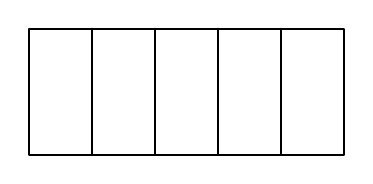
\begin{tikzpicture}[scale=0.8, line cap=round, line join=round]
  \draw[thick] (0,0) rectangle (5,2);
  \foreach \x in {1,2,3,4} {
    \draw[thick] (\x,0) -- (\x,2);
  }
\end{tikzpicture}
\end{center}
\nopagebreak[4]
\Needspace{4\baselineskip}
\textbf{解析}
\nopagebreak[4]
\begin{center}% 2003 年河南卷第 16 题：5 块并排试验田
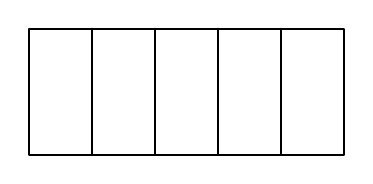
\begin{tikzpicture}[scale=0.8, line cap=round, line join=round]
  \draw[thick] (0,0) rectangle (5,2);
  \foreach \x in {1,2,3,4} {
    \draw[thick] (\x,0) -- (\x,2);
  }
\end{tikzpicture}
\end{center}
\nopagebreak[4]
5 块试验田自左向右依次编号为 1, 2, 3, 4, 5。每块种植一种作物，共 3 种不同作物，且相邻田块不能种植同一种作物：
\begin{itemize}
\item 第 1 块试验田有 3 种选择；
\item 第 2 块试验田不能与第 1 块相同，有 $3 - 1 = 2$ 种选择；
\item 第 3 块试验田不能与第 2 块相同，有 $3 - 1 = 2$ 种选择；
\item 第 4 块试验田不能与第 3 块相同，有 $3 - 1 = 2$ 种选择；
\item 第 5 块试验田不能与第 4 块相同，有 $3 - 1 = 2$ 种选择。
\end{itemize}
\Needspace{5\baselineskip}
根据分步乘法计数原理，不同的种植方法总数为：
\nopagebreak[4]
\[N = 3 \times 2 \times 2 \times 2 \times 2 = 3 \times 2^4 = 3 \times 16 = 48 \text{ \text{种}}.\]

\gkanswer{答案：48}

\end{answer}
\begin{answer}
\gksolhead{17}{}

\textbf{题目}：

已知函数 $f(x) = 2\sin x(\sin x + \cos x)$．
(1) 求函数 $f(x)$ 的最小正周期和最大值；
(2) 在给出的直角坐标系中，画出函数 $y = f(x)$ 在区间 $\left[-\dfrac{\pi}{2}, \dfrac{\pi}{2}\right]$ 上的图象．
\nopagebreak[4]
\begin{center}% 2003 年河南卷第 17 题：直角坐标系网格（题干图）
\begin{tikzpicture}[x=0.7cm,y=0.7cm,>=stealth]
  % Dashed grid
  \draw[dashed,thin] (-5,-5) grid (5,5);
  % Axes
  \draw[->,thick] (-5.6,0) -- (5.8,0) node[right] {\footnotesize $x$};
  \draw[->,thick] (0,-5.6) -- (0,5.8) node[above] {\footnotesize $y$};
  % Origin
  \node[above left] at (0,0) {\scriptsize $O$};
  
  % y-ticks and labels
  \node[left,fill=white,inner sep=0.5pt] at (0,1) {\tiny $\frac{1}{2}$};
  \node[left,fill=white,inner sep=0.5pt] at (0,2) {\tiny $1$};
  \node[left,fill=white,inner sep=0.5pt] at (0,3) {\tiny $\frac{3}{2}$};
  \node[left,fill=white,inner sep=0.5pt] at (0,4) {\tiny $2$};
  \node[left,fill=white,inner sep=0.5pt] at (0,5) {\tiny $\frac{5}{2}$};
  \node[left,fill=white,inner sep=0.5pt] at (0,-2) {\tiny $-1$};
  \node[left,fill=white,inner sep=0.5pt] at (0,-3) {\tiny $-\frac{3}{2}$};
  \node[left,fill=white,inner sep=0.5pt] at (0,-4) {\tiny $-2$};
  \node[left,fill=white,inner sep=0.5pt] at (0,-5) {\tiny $-\frac{5}{2}$};

  % x-ticks and labels
  \node[below,fill=white,inner sep=0.5pt] at (-5,0) {\tiny $-\frac{5\pi}{8}$};
  \node[below,fill=white,inner sep=0.5pt] at (-4,0) {\tiny $-\frac{\pi}{2}$};
  \node[below,fill=white,inner sep=0.5pt] at (-3,0) {\tiny $-\frac{3\pi}{8}$};
  \node[below,fill=white,inner sep=0.5pt] at (-2,0) {\tiny $-\frac{\pi}{4}$};
  \node[below,fill=white,inner sep=0.5pt] at (-1,0) {\tiny $-\frac{\pi}{8}$};
  \node[below,fill=white,inner sep=0.5pt] at (1,0) {\tiny $\frac{\pi}{8}$};
  \node[below,fill=white,inner sep=0.5pt] at (2,0) {\tiny $\frac{\pi}{4}$};
  \node[below,fill=white,inner sep=0.5pt] at (3,0) {\tiny $\frac{3\pi}{8}$};
  \node[below,fill=white,inner sep=0.5pt] at (4,0) {\tiny $\frac{\pi}{2}$};
  \node[below,fill=white,inner sep=0.5pt] at (5,0) {\tiny $\frac{5\pi}{8}$};
\end{tikzpicture}
\end{center}
\nopagebreak[4]
\Needspace{4\baselineskip}
\textbf{解析}

\Needspace{5\baselineskip}
由三角恒等变换：
\nopagebreak[4]
\[\begin{aligned}
f(x) &= 2\sin x(\sin x + \cos x) \\
&= 2\sin^2 x + 2\sin x\cos x \\
&= (1 - \cos 2x) + \sin 2x \\
&= 1 + \sin 2x - \cos 2x \\
&= 1 + \sqrt{2}\left(\frac{\sqrt{2}}{2}\sin 2x - \frac{\sqrt{2}}{2}\cos 2x\right) \\
&= 1 + \sqrt{2}\sin\left(2x - \frac{\pi}{4}\right).
\end{aligned}\]

\gksubpart{(1)}

\begin{itemize}
\item 函数 $f(x)$ 的最小正周期为：
\end{itemize}
\nopagebreak[4]
\[T = \frac{2\pi}{2} = \pi.\]
\begin{itemize}
\item 因为正弦函数的值域为 $[-1, 1]$，所以当 $\sin\left(2x - \dfrac{\pi}{4}\right) = 1$，即 $2x - \dfrac{\pi}{4} = 2k\pi + \dfrac{\pi}{2}$ ($k \in \mathbf{Z}$)，即 $x = k\pi + \dfrac{3\pi}{8}$ 时，函数 $f(x)$ 取得最大值：
\end{itemize}
\nopagebreak[4]
\[f_{\max} = 1 + \sqrt{2}.\]

\gksubpart{(2)}
\nopagebreak[4]
\begin{center}% 2003 年河南卷第 17 题：直角坐标系函数图象（解析答案图）
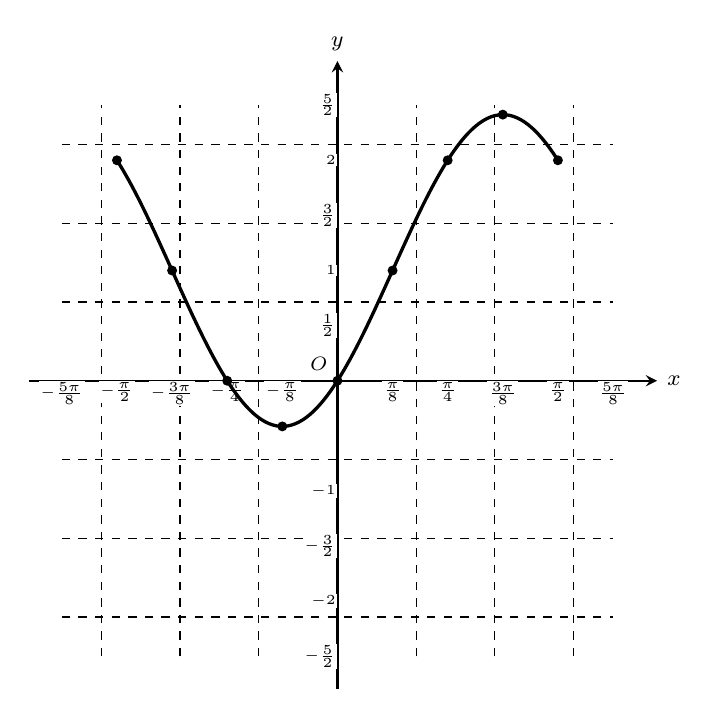
\begin{tikzpicture}[x=0.7cm,y=0.7cm,>=stealth]
  % Dashed grid
  \draw[dashed,thin] (-5,-5) grid (5,5);
  % Axes
  \draw[->,thick] (-5.6,0) -- (5.8,0) node[right] {\footnotesize $x$};
  \draw[->,thick] (0,-5.6) -- (0,5.8) node[above] {\footnotesize $y$};
  % Origin
  \node[above left] at (0,0) {\scriptsize $O$};
  
  % y-ticks and labels
  \node[left,fill=white,inner sep=0.5pt] at (0,1) {\tiny $\frac{1}{2}$};
  \node[left,fill=white,inner sep=0.5pt] at (0,2) {\tiny $1$};
  \node[left,fill=white,inner sep=0.5pt] at (0,3) {\tiny $\frac{3}{2}$};
  \node[left,fill=white,inner sep=0.5pt] at (0,4) {\tiny $2$};
  \node[left,fill=white,inner sep=0.5pt] at (0,5) {\tiny $\frac{5}{2}$};
  \node[left,fill=white,inner sep=0.5pt] at (0,-2) {\tiny $-1$};
  \node[left,fill=white,inner sep=0.5pt] at (0,-3) {\tiny $-\frac{3}{2}$};
  \node[left,fill=white,inner sep=0.5pt] at (0,-4) {\tiny $-2$};
  \node[left,fill=white,inner sep=0.5pt] at (0,-5) {\tiny $-\frac{5}{2}$};

  % x-ticks and labels
  \node[below,fill=white,inner sep=0.5pt] at (-5,0) {\tiny $-\frac{5\pi}{8}$};
  \node[below,fill=white,inner sep=0.5pt] at (-4,0) {\tiny $-\frac{\pi}{2}$};
  \node[below,fill=white,inner sep=0.5pt] at (-3,0) {\tiny $-\frac{3\pi}{8}$};
  \node[below,fill=white,inner sep=0.5pt] at (-2,0) {\tiny $-\frac{\pi}{4}$};
  \node[below,fill=white,inner sep=0.5pt] at (-1,0) {\tiny $-\frac{\pi}{8}$};
  \node[below,fill=white,inner sep=0.5pt] at (1,0) {\tiny $\frac{\pi}{8}$};
  \node[below,fill=white,inner sep=0.5pt] at (2,0) {\tiny $\frac{\pi}{4}$};
  \node[below,fill=white,inner sep=0.5pt] at (3,0) {\tiny $\frac{3\pi}{8}$};
  \node[below,fill=white,inner sep=0.5pt] at (4,0) {\tiny $\frac{\pi}{2}$};
  \node[below,fill=white,inner sep=0.5pt] at (5,0) {\tiny $\frac{5\pi}{8}$};

  % Plotted curve
  \draw[very thick,domain=-4:4,samples=120,smooth] plot (\x, {2 + 2*sqrt(2)*sin(45*\x - 45)});
  % Key points
  \foreach \coord in {(-4,4), (-3,2), (-2,0), (-1,{2-2*sqrt(2)}), (0,0), (1,2), (2,4), (3,{2+2*sqrt(2)}), (4,4)} {
    \fill \coord circle (1.8pt);
  }
\end{tikzpicture}
\end{center}
\nopagebreak[4]
在区间 $\left[-\dfrac{\pi}{2}, \dfrac{\pi}{2}\right]$ 上，列出关键点坐标：
\begin{itemize}
\item 当 $x = -\dfrac{\pi}{2}$ 时，$2x - \dfrac{\pi}{4} = -\dfrac{5\pi}{4}$，$\sin\left(-\dfrac{5\pi}{4}\right) = \dfrac{\sqrt{2}}{2}$，故 $f\left(-\dfrac{\pi}{2}\right) = 1 + \sqrt{2} \times \dfrac{\sqrt{2}}{2} = 2$；
\item 当 $x = -\dfrac{3\pi}{8}$ 时，$2x - \dfrac{\pi}{4} = -\pi$，故 $f\left(-\dfrac{3\pi}{8}\right) = 1 + 0 = 1$；
\item 当 $x = -\dfrac{\pi}{4}$ 时，$2x - \dfrac{\pi}{4} = -\dfrac{3\pi}{4}$，故 $f\left(-\dfrac{\pi}{4}\right) = 1 - 1 = 0$；
\item 当 $x = -\dfrac{\pi}{8}$ 时，$2x - \dfrac{\pi}{4} = -\dfrac{\pi}{2}$，故 $f\left(-\dfrac{\pi}{8}\right) = 1 - \sqrt{2} \approx -0.414$（极小值点）；
\item 当 $x = 0$ 时，$2x - \dfrac{\pi}{4} = -\dfrac{\pi}{4}$，故 $f(0) = 1 - 1 = 0$；
\item 当 $x = \dfrac{\pi}{8}$ 时，$2x - \dfrac{\pi}{4} = 0$，故 $f\left(\dfrac{\pi}{8}\right) = 1 + 0 = 1$；
\item 当 $x = \dfrac{\pi}{4}$ 时，$2x - \dfrac{\pi}{4} = \dfrac{\pi}{4}$，故 $f\left(\dfrac{\pi}{4}\right) = 1 + 1 = 2$；
\item 当 $x = \dfrac{3\pi}{8}$ 时，$2x - \dfrac{\pi}{4} = \dfrac{\pi}{2}$，故 $f\left(\dfrac{3\pi}{8}\right) = 1 + \sqrt{2} \approx 2.414$（极大值点）；
\item 当 $x = \dfrac{\pi}{2}$ 时，$2x - \dfrac{\pi}{4} = \dfrac{3\pi}{4}$，故 $f\left(\dfrac{\pi}{2}\right) = 1 + 1 = 2$。
\end{itemize}

在给出的直角坐标系中，依次描出上述各点，并用平滑曲线连接，即得函数 $y = f(x)$ 在 $\left[-\dfrac{\pi}{2}, \dfrac{\pi}{2}\right]$ 上的完整图象。

\gkanswer{答案（1）：最小正周期为 $\pi$，最大值为 $1 + \sqrt{2}$}

\gkanswer{答案（2）：作图见解析}

\end{answer}
\begin{answer}
\gksolhead{18}{}

\textbf{题目}：

有三种产品，合格率分别是 0.90，0.95 和 0.95，各抽取一件进行检验．
(1) 求恰有一件不合格的概率；
(2) 求至少有两件不合格的概率．（精确到 0.001）

\Needspace{4\baselineskip}
\textbf{解析}

记事件 $A_1, A_2, A_3$ 分别表示抽到的第一、二、三件产品为合格品，则 $A_1, A_2, A_3$ 相互独立。
\Needspace{5\baselineskip}
已知：
\nopagebreak[4]
\[P(A_1) = 0.90, \quad P(A_2) = 0.95, \quad P(A_3) = 0.95.\]
\Needspace{5\baselineskip}
对应的不合格概率分别为：
\nopagebreak[4]
\[P(\bar{A}_1) = 1 - 0.90 = 0.10, \quad P(\bar{A}_2) = 1 - 0.95 = 0.05, \quad P(\bar{A}_3) = 1 - 0.95 = 0.05.\]

\gksubpart{(1)}

恰有一件不合格包含三种互斥情况：只有第一件不合格、只有第二件不合格、只有第三件不合格。
\Needspace{5\baselineskip}
其概率为：
\nopagebreak[4]
\[\begin{aligned}
P_1 &= P(\bar{A}_1 A_2 A_3) + P(A_1 \bar{A}_2 A_3) + P(A_1 A_2 \bar{A}_3) \\
&= 0.10 \times 0.95 \times 0.95 + 0.90 \times 0.05 \times 0.95 + 0.90 \times 0.95 \times 0.05 \\
&= 0.10 \times 0.9025 + 0.04275 + 0.04275 \\
&= 0.09025 + 0.0855 \\
&= 0.17575.
\end{aligned}\]
答：恰有一件不合格的概率为 $0.17575$。

\gksubpart{(2)}

“至少有两件不合格”的对立事件是“全合格”以及“恰有一件不合格”。
\Needspace{5\baselineskip}
全部合格的概率为：
\nopagebreak[4]
\[P_0 = P(A_1 A_2 A_3) = 0.90 \times 0.95 \times 0.95 = 0.90 \times 0.9025 = 0.81225.\]
\Needspace{5\baselineskip}
因此，至少有两件不合格的概率为：
\nopagebreak[4]
\[\begin{aligned}
P_{\ge 2} &= 1 - P_0 - P_1 \\
&= 1 - 0.81225 - 0.17575 \\
&= 1 - 0.98800 \\
&= 0.012.
\end{aligned}\]
答：至少有两件不合格的概率精确到 0.001 为 $0.012$。

\gkanswer{答案（1）：$0.17575$}

\gkanswer{答案（2）：$0.012$}

\end{answer}
\begin{answer}
\gksolhead{19}{}

\textbf{题目}：

如图，在直三棱柱 $ABC - A_1B_1C_1$ 中，底面是等腰直角三角形，$\angle ACB = 90^\circ$，侧棱 $AA_1 = 2$，$D$、$E$ 分别是 $CC_1$ 与 $A_1B$ 的中点，点 $E$ 在平面 $ABD$ 上的射影是 $\triangle ABD$ 的重心 $G$．
(1) 求 $A_1B$ 与平面 $ABD$ 所成角的大小（结果用反三角函数值表示）；
(2) 求点 $A_1$ 到平面 $AED$ 的距离．
\nopagebreak[4]
\begin{center}% 2003 年河南卷第 19 题：直三棱柱立体几何图
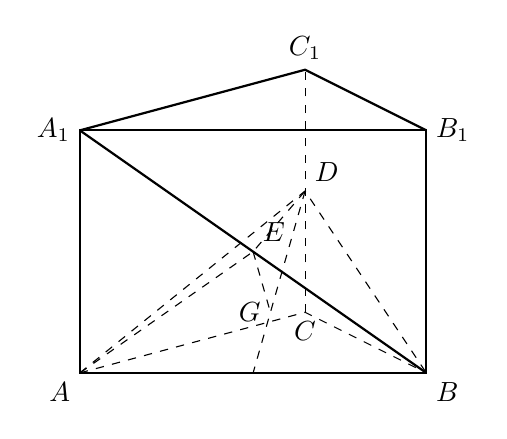
\begin{tikzpicture}[>=stealth,scale=1.1]
  % Vertices
  \coordinate (A) at (0,0);
  \coordinate (B) at (4,0);
  \coordinate (A1) at (0,2.8);
  \coordinate (B1) at (4,2.8);
  \coordinate (C) at (2.6,0.7);
  \coordinate (C1) at (2.6,3.5);
  
  \coordinate (D) at (2.6,2.1); % midpoint of CC1
  \coordinate (E) at (2,1.4);   % midpoint of A1B
  
  \coordinate (M) at (2,0);     % midpoint of AB
  \coordinate (G) at (2.2,0.7); % centroid of ABD on median DM
  
  % Solid visible edges of prism
  \draw[thick] (A) -- (B) -- (B1) -- (A1) -- cycle;
  \draw[thick] (A1) -- (C1) -- (B1);
  \draw[thick] (A1) -- (B); % diagonal
  
  % Dashed edges of prism
  \draw[dashed] (A) -- (C) -- (B);
  \draw[dashed] (C) -- (D) -- (C1);
  
  % Dashed lines for problem geometry
  \draw[dashed] (A) -- (D) -- (B);
  \draw[dashed] (A) -- (E) -- (D);
  \draw[dashed] (E) -- (G);
  \draw[dashed] (D) -- (M);
  
  % Labels
  \node[below left] at (A) {$A$};
  \node[below right] at (B) {$B$};
  \node[left] at (A1) {$A_1$};
  \node[right] at (B1) {$B_1$};
  \node[below] at (C) {$C$};
  \node[above] at (C1) {$C_1$};
  \node[above right] at (D) {$D$};
  \node[above right] at (E) {$E$};
  \node[left] at (G) {$G$};
\end{tikzpicture}
\end{center}
\nopagebreak[4]
\Needspace{4\baselineskip}
\textbf{解析}
\nopagebreak[4]
\begin{center}% 2003 年河南卷第 19 题：直三棱柱立体几何图
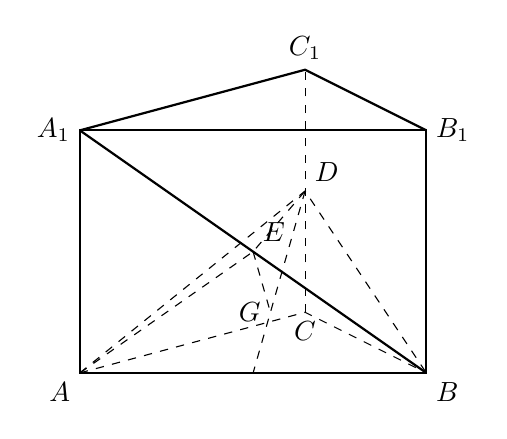
\begin{tikzpicture}[>=stealth,scale=1.1]
  % Vertices
  \coordinate (A) at (0,0);
  \coordinate (B) at (4,0);
  \coordinate (A1) at (0,2.8);
  \coordinate (B1) at (4,2.8);
  \coordinate (C) at (2.6,0.7);
  \coordinate (C1) at (2.6,3.5);
  
  \coordinate (D) at (2.6,2.1); % midpoint of CC1
  \coordinate (E) at (2,1.4);   % midpoint of A1B
  
  \coordinate (M) at (2,0);     % midpoint of AB
  \coordinate (G) at (2.2,0.7); % centroid of ABD on median DM
  
  % Solid visible edges of prism
  \draw[thick] (A) -- (B) -- (B1) -- (A1) -- cycle;
  \draw[thick] (A1) -- (C1) -- (B1);
  \draw[thick] (A1) -- (B); % diagonal
  
  % Dashed edges of prism
  \draw[dashed] (A) -- (C) -- (B);
  \draw[dashed] (C) -- (D) -- (C1);
  
  % Dashed lines for problem geometry
  \draw[dashed] (A) -- (D) -- (B);
  \draw[dashed] (A) -- (E) -- (D);
  \draw[dashed] (E) -- (G);
  \draw[dashed] (D) -- (M);
  
  % Labels
  \node[below left] at (A) {$A$};
  \node[below right] at (B) {$B$};
  \node[left] at (A1) {$A_1$};
  \node[right] at (B1) {$B_1$};
  \node[below] at (C) {$C$};
  \node[above] at (C1) {$C_1$};
  \node[above right] at (D) {$D$};
  \node[above right] at (E) {$E$};
  \node[left] at (G) {$G$};
\end{tikzpicture}
\end{center}
\nopagebreak[4]
在直三棱柱 $ABC-A_1B_1C_1$ 中，侧棱垂直于底面。
底面 $\triangle ABC$ 为等腰直角三角形，$\angle ACB = 90^\circ$，设 $CA = CB = a$。
\Needspace{5\baselineskip}
建立空间直角坐标系，以 $C$ 为原点，$CA, CB, CC_1$ 所在直线分别为 $x, y, z$ 轴：
\nopagebreak[4]
\[C(0, 0, 0), \quad A(a, 0, 0), \quad B(0, a, 0), \quad C_1(0, 0, 2), \quad A_1(a, 0, 2), \quad B_1(0, a, 2).\]
\Needspace{5\baselineskip}
因为 $D, E$ 分别是 $CC_1$ 与 $A_1B$ 的中点，所以：
\nopagebreak[4]
\[D(0, 0, 1), \quad E\left(\frac{a}{2}, \frac{a}{2}, 1\right).\]
\Needspace{5\baselineskip}
$\triangle ABD$ 的顶点坐标为 $A(a, 0, 0), B(0, a, 0), D(0, 0, 1)$，其重心 $G$ 的坐标为：
\nopagebreak[4]
\[G = \left(\frac{a + 0 + 0}{3}, \frac{0 + a + 0}{3}, \frac{0 + 0 + 1}{3}\right) = \left(\frac{a}{3}, \frac{a}{3}, \frac{1}{3}\right).\]
\Needspace{5\baselineskip}
向量 $\vec{EG}$ 为：
\nopagebreak[4]
\[\vec{EG} = G - E = \left(\frac{a}{3} - \frac{a}{2}, \frac{a}{3} - \frac{a}{2}, \frac{1}{3} - 1\right) = \left(-\frac{a}{6}, -\frac{a}{6}, -\frac{2}{3}\right).\]
因为点 $E$ 在平面 $ABD$ 上的射影是 $G$，所以 $EG \perp \text{\text{平面} } ABD$。
平面 $ABD$ 的一个法向量可取为 $\vec{n} = 6\vec{EG} = (-a, -a, -4)$。
\Needspace{5\baselineskip}
又向量 $\vec{DA} = (a, 0, -1)$ 在平面 $ABD$ 内，由 $\vec{n} \cdot \vec{DA} = 0$ 得：
\nopagebreak[4]
\[-a \cdot a + (-a) \cdot 0 + (-4) \cdot (-1) = 0 \implies -a^2 + 4 = 0.\]
因为 $a > 0$，所以 $a = 2$。
\Needspace{5\baselineskip}
此时各点坐标确定为：
\nopagebreak[4]
\[A(2, 0, 0), \quad B(0, 2, 0), \quad D(0, 0, 1), \quad A_1(2, 0, 2), \quad E(1, 1, 1), \quad G\left(\frac{2}{3}, \frac{2}{3}, \frac{1}{3}\right).\]
法向量 $\vec{n} = (-2, -2, -4)$，化简可取平面 $ABD$ 的单位法向量或直接使用 $\vec{m} = (1, 1, 2)$。

\gksubpart{(1)}

向量 $\vec{A_1B} = B - A_1 = (-2, 2, -2)$。
因为 $EG \perp \text{\text{平面} } ABD$，所以 $\vec{m} = (1, 1, 2)$ 为平面 $ABD$ 的法向量。
\Needspace{5\baselineskip}
设 $A_1B$ 与平面 $ABD$ 所成角为 $\theta$（$0 \le \theta \le \dfrac{\pi}{2}$），则：
\nopagebreak[4]
\[\sin\theta = \frac{|\vec{A_1B} \cdot \vec{m}|}{|\vec{A_1B}| \cdot |\vec{m}|} = \frac{|(-2) \times 1 + 2 \times 1 + (-2) \times 2|}{\sqrt{(-2)^2 + 2^2 + (-2)^2} \cdot \sqrt{1^2 + 1^2 + 2^2}} = \frac{|-4|}{\sqrt{12} \cdot \sqrt{6}} = \frac{4}{6\sqrt{2}} = \frac{\sqrt{2}}{3}.\]
所以 $A_1B$ 与平面 $ABD$ 所成角的大小为 $\arcsin\dfrac{\sqrt{2}}{3}$。

\gksubpart{(2)}

\Needspace{5\baselineskip}
在平面 $AED$ 中：
\nopagebreak[4]
\[A(2, 0, 0), \quad E(1, 1, 1), \quad D(0, 0, 1).\]
向量 $\vec{DA} = (2, 0, -1)$，$\vec{DE} = (1, 1, 0)$。
\Needspace{5\baselineskip}
设平面 $AED$ 的法向量为 $\vec{n}_1 = (x, y, z)$，则：
\nopagebreak[4]
\[\begin{cases} 2x - z = 0, \\ x + y = 0. \end{cases}\]
取 $x = 1$，则 $y = -1$，$z = 2$。故 $\vec{n}_1 = (1, -1, 2)$。
向量 $\vec{DA_1} = A_1 - D = (2, 0, 2) - (0, 0, 1) = (2, 0, 1)$。
\Needspace{5\baselineskip}
点 $A_1$ 到平面 $AED$ 的距离为：
\nopagebreak[4]
\[d = \frac{|\vec{DA_1} \cdot \vec{n}_1|}{|\vec{n}_1|} = \frac{|2 \times 1 + 0 \times (-1) + 1 \times 2|}{\sqrt{1^2 + (-1)^2 + 2^2}} = \frac{4}{\sqrt{6}} = \frac{2\sqrt{6}}{3}.\]

\gkanswer{答案（1）：$\arcsin\dfrac{\sqrt{2}}{3}$}

\gkanswer{答案（2）：$\dfrac{2\sqrt{6}}{3}$}

\end{answer}
\begin{answer}
\gksolhead{20}{}

\textbf{题目}：

已知 $c > 0$，设 $P$：函数 $y = c^x$ 在 $\mathbf{R}$ 上单调递减；$Q$：不等式 $x + |x - 2c| > 1$ 的解集为 $\mathbf{R}$．如果 $P$ 和 $Q$ 有且仅有一个正确，求 $c$ 的取值范围．

\Needspace{4\baselineskip}
\textbf{解析}

命题 $P$：函数 $y = c^x$ 在 $\mathbf{R}$ 上单调递减。
\Needspace{5\baselineskip}
根据指数函数的单调性质，底数满足：
\nopagebreak[4]
\[0 < c < 1.\]
故命题 $P$ 为真时 $c \in (0, 1)$；$P$ 为假时 $c \in [1, +\infty)$。

命题 $Q$：不等式 $x + |x - 2c| > 1$ 的解集为 $\mathbf{R}$。
\Needspace{5\baselineskip}
考察函数 $g(x) = x + |x - 2c|$：
\nopagebreak[4]
\[g(x) = \begin{cases} 2x - 2c, & x \ge 2c, \\ 2c, & x < 2c. \end{cases}\]
\begin{itemize}
\item 当 $x < 2c$ 时，$g(x) = 2c$；
\item 当 $x \ge 2c$ 时，$g(x) = 2x - 2c \ge 4c - 2c = 2c$。
\end{itemize}
因此，函数 $g(x)$ 在 $\mathbf{R}$ 上的最小值为 $2c$。
\Needspace{5\baselineskip}
不等式 $x + |x - 2c| > 1$ 的解集为 $\mathbf{R}$，当且仅当其最小值大于 1：
\nopagebreak[4]
\[\min g(x) = 2c > 1 \iff c > \frac{1}{2}.\]
故命题 $Q$ 为真时 $c \in \left(\dfrac{1}{2}, +\infty\right)$；$Q$ 为假时 $c \in \left(0, \dfrac{1}{2}\right]$。

根据题意，“$P$ 和 $Q$ 有且仅有一个正确”，分两种情况讨论：
\Needspace{5\baselineskip}
1. \textbf{$P$ 真且 $Q$ 假}：
\nopagebreak[4]
\[\begin{cases} 0 < c < 1, \\ 0 < c \le \dfrac{1}{2}, \end{cases} \implies 0 < c \le \frac{1}{2}.\]
\Needspace{5\baselineskip}
2. \textbf{$P$ 假且 $Q$ 真}：
\nopagebreak[4]
\[\begin{cases} c \ge 1, \\ c > \dfrac{1}{2}, \end{cases} \implies c \ge 1.\]

综上所述，$c$ 的取值范围为 $\left(0, \dfrac{1}{2}\right] \cup [1, +\infty)$。

\gkanswer{答案：$\left(0, \dfrac{1}{2}\right] \cup [1, +\infty)$}

\end{answer}
\begin{answer}
\gksolhead{21}{}

\textbf{题目}：

已知常数 $a > 0$，向量 $\vec{c} = (0, a)$，$\vec{i} = (1, 0)$，经过原点 $O$ 以 $\vec{c} + \lambda\vec{i}$ 为方向向量的直线与经过定点 $A(0, a)$ 以 $\vec{i} - 2\lambda\vec{c}$ 为方向向量的直线相交于点 $P$，其中 $\lambda \in \mathbf{R}$．
试问：是否存在两个定点 $E$、$F$，使得 $|PE| + |PF|$ 为定值．若存在，求出 $E$、$F$ 的坐标；若不存在，说明理由．

\Needspace{4\baselineskip}
\textbf{解析}

已知向量 $\vec{c} = (0, a)$，$\vec{i} = (1, 0)$，其中 $a > 0$。
\begin{itemize}
\item 直线 $l_1$ 经过原点 $O(0, 0)$，方向向量为 $\vec{c} + \lambda\vec{i} = (\lambda, a)$。
\end{itemize}
\Needspace{5\baselineskip}
  当 $\lambda \ne 0$ 时，直线的斜率为 $\dfrac{a}{\lambda}$，方程为：
\nopagebreak[4]
\[y = \frac{a}{\lambda} x \iff ax - \lambda y = 0.\]
  当 $\lambda = 0$ 时，方向向量为 $(0, a)$，直线为 $y$ 轴（$x = 0$），也满足上式。
\begin{itemize}
\item 直线 $l_2$ 经过定点 $A(0, a)$，方向向量为 $\vec{i} - 2\lambda\vec{c} = (1, -2\lambda a)$。
\end{itemize}
\Needspace{5\baselineskip}
  直线的斜率为 $-2\lambda a$，方程为：
\nopagebreak[4]
\[y - a = -2\lambda a x \iff 2\lambda a x + y - a = 0.\]
设直线 $l_1$ 与 $l_2$ 相交于点 $P(x, y)$。
由 $ax - \lambda y = 0$：
当 $y \ne 0$ 时，$\lambda = \dfrac{ax}{y}$。
\Needspace{5\baselineskip}
将其代入 $l_2$ 的方程中：
\nopagebreak[4]
\[2\left(\frac{ax}{y}\right) a x + y - a = 0 \implies \frac{2a^2 x^2}{y} + y - a = 0.\]
\Needspace{5\baselineskip}
两边同乘以 $y$ 并整理：
\nopagebreak[4]
\[2a^2 x^2 + y^2 - ay = 0.\]
\Needspace{5\baselineskip}
配方得：
\nopagebreak[4]
\[2a^2 x^2 + \left(y - \frac{a}{2}\right)^2 = \frac{a^2}{4}.\]
\Needspace{5\baselineskip}
两边同除以 $\dfrac{a^2}{4}$：
\nopagebreak[4]
\[\frac{x^2}{\dfrac{1}{8}} + \frac{\left(y - \dfrac{a}{2}\right)^2}{\dfrac{a^2}{4}} = 1.\]
（检验 $\lambda = 0$ 时，交点为 $(0, a)$，满足方程；当 $\lambda \to \infty$ 时交点趋近 $(0, 0)$）。
此方程表示中心在 $\left(0, \dfrac{a}{2}\right)$ 的二次曲线，根据椭圆第一定义，存在两个定点 $E, F$ 使得 $|PE| + |PF|$ 为定值。
比较两分母 $\dfrac{a^2}{4}$ 与 $\dfrac{1}{8}$ 的大小：

1. 当 $\dfrac{a^2}{4} > \dfrac{1}{8}$，即 $a > \dfrac{\sqrt{2}}{2}$ 时：
   曲线是长轴在直线 $x = 0$ 上的椭圆。
\Needspace{5\baselineskip}
   长半轴长为 $A = \dfrac{a}{2}$，半焦距为：
\nopagebreak[4]
\[c_0 = \sqrt{\frac{a^2}{4} - \frac{1}{8}} = \frac{\sqrt{4a^2 - 2}}{4}.\]
\Needspace{5\baselineskip}
   焦点在 $y$ 轴上，坐标为：
\nopagebreak[4]
\[E\left(0, \frac{a}{2} - \frac{\sqrt{4a^2 - 2}}{4}\right), \quad F\left(0, \frac{a}{2} + \frac{\sqrt{4a^2 - 2}}{4}\right).\]
   此时 $|PE| + |PF| = 2A = a$ 为定值。

2. 当 $\dfrac{a^2}{4} = \dfrac{1}{8}$，即 $a = \dfrac{\sqrt{2}}{2}$ 时：
   方程化为 $x^2 + \left(y - \dfrac{\sqrt{2}}{4}\right)^2 = \dfrac{1}{8}$，轨迹为圆。
   两焦点重合于圆心 $\left(0, \dfrac{\sqrt{2}}{4}\right)$，取 $E = F = \left(0, \dfrac{\sqrt{2}}{4}\right)$，
   此时 $|PE| + |PF| = 2|PE| = 2 \times \dfrac{\sqrt{2}}{4} = \dfrac{\sqrt{2}}{2}$ 为定值。

3. 当 $\dfrac{a^2}{4} < \dfrac{1}{8}$，即 $0 < a < \dfrac{\sqrt{2}}{2}$ 时：
   曲线是长轴在直线 $y = \dfrac{a}{2}$ 上的椭圆。
\Needspace{5\baselineskip}
   长半轴长为 $A = \dfrac{\sqrt{2}}{4}$，半焦距为：
\nopagebreak[4]
\[c_0 = \sqrt{\frac{1}{8} - \frac{a^2}{4}} = \frac{\sqrt{2 - 4a^2}}{4}.\]
\Needspace{5\baselineskip}
   焦点坐标为：
\nopagebreak[4]
\[E\left(-\frac{\sqrt{2 - 4a^2}}{4}, \frac{a}{2}\right), \quad F\left(\frac{\sqrt{2 - 4a^2}}{4}, \frac{a}{2}\right).\]
   此时 $|PE| + |PF| = 2A = \dfrac{\sqrt{2}}{2}$ 为定值。

\gkanswer{答案：存在。当 $a > \dfrac{\sqrt{2}}{2}$ 时，$E\left(0, \dfrac{a}{2} - \dfrac{\sqrt{4a^2 - 2}}{4}\right)$，$F\left(0, \dfrac{a}{2} + \dfrac{\sqrt{4a^2 - 2}}{4}\right)$，定值为 $a$；当 $a = \dfrac{\sqrt{2}}{2}$ 时，$E, F$ 重合于点 $\left(0, \dfrac{\sqrt{2}}{4}\right)$，定值为 $\dfrac{\sqrt{2}}{2}$；当 $0 < a < \dfrac{\sqrt{2}}{2}$ 时，$E\left(-\dfrac{\sqrt{2 - 4a^2}}{4}, \dfrac{a}{2}\right)$，$F\left(\dfrac{\sqrt{2 - 4a^2}}{4}, \dfrac{a}{2}\right)$，定值为 $\dfrac{\sqrt{2}}{2}$。}

\end{answer}
\begin{answer}
\gksolhead{22}{}

\textbf{题目}：

已知 $a > 0$，$n$ 为正整数．
(1) 设 $y = (x - a)^n$，证明 $y' = n(x - a)^{n-1}$；
(2) 设 $f_n(x) = x^n - (x - a)^n$，对任意 $n \ge a$，证明 $f_{n+1}'(n+1) > (n+1)f_n'(n)$．

\Needspace{4\baselineskip}
\textbf{解析}

\gksubpart{(1)}

\textbf{证法一（导数定义）}：
\Needspace{5\baselineskip}
由导数定义：
\nopagebreak[4]
\[y' = \lim_{\Delta x \to 0} \frac{(x + \Delta x - a)^n - (x - a)^n}{\Delta x}.\]
\Needspace{5\baselineskip}
令 $u = x - a$，利用二项式定理展开 $(u + \Delta x)^n$：
\nopagebreak[4]
\[(u + \Delta x)^n = u^n + n u^{n-1} \Delta x + \binom{n}{2} u^{n-2} (\Delta x)^2 + \cdots + (\Delta x)^n.\]
\Needspace{5\baselineskip}
代入差商：
\nopagebreak[4]
\[\frac{(u + \Delta x)^n - u^n}{\Delta x} = n u^{n-1} + \binom{n}{2} u^{n-2} \Delta x + \cdots + (\Delta x)^{n-1}.\]
\Needspace{5\baselineskip}
取极限 $\Delta x \to 0$：
\nopagebreak[4]
\[y' = \lim_{\Delta x \to 0} \left[ n u^{n-1} + \binom{n}{2} u^{n-2} \Delta x + \cdots + (\Delta x)^{n-1} \right] = n u^{n-1} = n(x - a)^{n-1}.\]

\textbf{证法二（二项式定理求导）}：
\Needspace{5\baselineskip}
将 $(x - a)^n$ 展开：
\nopagebreak[4]
\[(x - a)^n = \sum_{k=0}^n \binom{n}{k} x^k (-a)^{n-k}.\]
\Needspace{5\baselineskip}
逐项求导：
\nopagebreak[4]
\[y' = \sum_{k=1}^n \binom{n}{k} k x^{k-1} (-a)^{n-k}.\]
\Needspace{5\baselineskip}
利用组合恒等式 $k \binom{n}{k} = n \binom{n-1}{k-1}$：
\nopagebreak[4]
\[y' = n \sum_{k=1}^n \binom{n-1}{k-1} x^{k-1} (-a)^{n-k} = n \sum_{j=0}^{n-1} \binom{n-1}{j} x^j (-a)^{n-1-j} = n(x - a)^{n-1}.\]

\gksubpart{(2)}

\Needspace{5\baselineskip}
由 (1) 的结论，对 $f_n(x) = x^n - (x - a)^n$ 求导：
\nopagebreak[4]
\[f_n'(x) = n x^{n-1} - n(x - a)^{n-1} = n [x^{n-1} - (x - a)^{n-1}].\]
\Needspace{5\baselineskip}
从而：
\nopagebreak[4]
\[(n + 1) f_n'(n) = n(n + 1) [n^{n-1} - (n - a)^{n-1}].\]
\Needspace{5\baselineskip}
同理，将 $n$ 换为 $n + 1$：
\nopagebreak[4]
\[f_{n+1}'(x) = (n + 1) [x^n - (x - a)^n].\]
\Needspace{5\baselineskip}
代入 $x = n + 1$：
\nopagebreak[4]
\[f_{n+1}'(n + 1) = (n + 1) [(n + 1)^n - (n + 1 - a)^n].\]
\Needspace{5\baselineskip}
要证明 $f_{n+1}'(n + 1) > (n + 1) f_n'(n)$，由于 $n + 1 > 0$，等价于证明：
\nopagebreak[4]
\[(n + 1)^n - (n + 1 - a)^n > n [n^{n-1} - (n - a)^{n-1}] = n^n - n(n - a)^{n-1}.\]
\Needspace{5\baselineskip}
移项整理，即证：
\nopagebreak[4]
\[(n + 1)^n - n^n > (n + 1 - a)^n - n(n - a)^{n-1}.\]
\Needspace{5\baselineskip}
考查右边式子：
\nopagebreak[4]
\[\begin{aligned}
(n + 1 - a)^n - n(n - a)^{n-1} &= [(n + 1 - a)^n - (n - a)^n] + [(n - a)^n - n(n - a)^{n-1}] \\
&= [(n + 1 - a)^n - (n - a)^n] + (n - a - n)(n - a)^{n-1} \\
&= [(n + 1 - a)^n - (n - a)^n] - a(n - a)^{n-1}.
\end{aligned}\]
因为已知 $a > 0$ 且 $n \ge a \implies n - a \ge 0$，所以 $a(n - a)^{n-1} \ge 0$。
\Needspace{5\baselineskip}
从而：
\nopagebreak[4]
\[(n + 1 - a)^n - n(n - a)^{n-1} \le (n + 1 - a)^n - (n - a)^n.\]
特别地，当 $n > a$ 时，$a(n - a)^{n-1} > 0$，有严格不等式；
当 $n = a$ 时，$n - a = 0$：
右边 $= 1^n - n \times 0 = 1$；
左边 $= (n + 1)^n - n^n$。当 $n \ge 1$ 时，由二项式展开 $(n + 1)^n - n^n \ge n \cdot n^{n-1} \ge 1$，严格大于 1。
再考查函数 $g(t) = t^n$ 在 $t \ge 0$ 上的性质：
其导函数 $g'(t) = n t^{n-1}$ 在 $[0, +\infty)$ 上单调递增（当 $n \ge 2$ 时严格单调递增；当 $n = 1$ 时可直接验证）。
\Needspace{5\baselineskip}
由拉格朗日中值定理，存在 $\xi_1 \in (n - a, n + 1 - a)$ 和 $\xi_2 \in (n, n + 1)$，使得：
\nopagebreak[4]
\[(n + 1 - a)^n - (n - a)^n = g'(\xi_1) = n \xi_1^{n-1},\]
\nopagebreak[4]
\[(n + 1)^n - n^n = g'(\xi_2) = n \xi_2^{n-1}.\]
因为 $a > 0$，所以区间 $[n - a, n + 1 - a]$ 严格位于 $[n, n + 1]$ 的左侧，故 $\xi_1 < \xi_2$。
\Needspace{5\baselineskip}
由导函数的单调递增性可知：
\nopagebreak[4]
\[(n + 1 - a)^n - (n - a)^n \le (n + 1)^n - n^n.\]
\Needspace{5\baselineskip}
结合前面的放缩：
\nopagebreak[4]
\[(n + 1 - a)^n - n(n - a)^{n-1} \le [(n + 1 - a)^n - (n - a)^n] - a(n - a)^{n-1} < (n + 1)^n - n^n.\]
\Needspace{5\baselineskip}
从而原不等式成立：
\nopagebreak[4]
\[f_{n+1}'(n + 1) > (n + 1) f_n'(n).\]
证毕。

\gkanswer{答案（1）：证明见解析}

\gkanswer{答案（2）：证明见解析}

\end{answer}